%! Author = Philipp Emmenegger
%! Date = 09/07/2021

\section{React}
\begin{itemize}
    \item Library, kein Framework
    \item Um User Interfaces zu bauen
    \item View in MVC
    \item Minimales Featureset
    \item Entwickelt von Facebook
    \item Verwendet für: WhatsApp, Insta, AirBnb, etc.
\end{itemize}
\subsubsection{Prinzipien}
\begin{itemize}
    \item Komplexes Problem aufteilen in einfachere Komponenten
    \item Für eine bessere: Wiederverwendbarkeit, Erweiterbarkeit, Wartbarkeit, Testbarkeit, Aufgabenverteilung
\end{itemize}

\subsection{Entwicklung von UIs}
\begin{itemize}
    \item Beschreibung des UIs
    \item Event-Handling
    \item Aktualisieren der Views
\end{itemize}

\subsection{Komponenten und Elemente}
\begin{itemize}
    \item Funktionen die HTML zurückgeben
    \item Beliebige Komposition von React-Elementen und DOM-Elementen
\end{itemize}
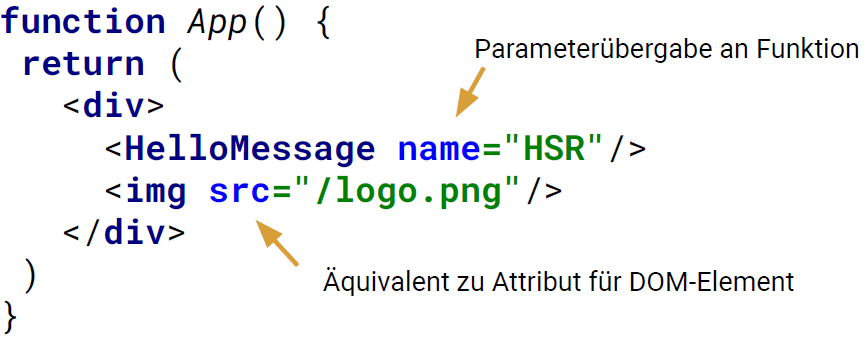
\includegraphics[width=0.6\linewidth]{img/react_component.png}

\subsection{JavaScript XML}
React verwendet JSX (blau), eine Erweiterung von JavaScript (gelb).
Überall wo JSX verwendet wird, muss $react$ importiert werden.\\
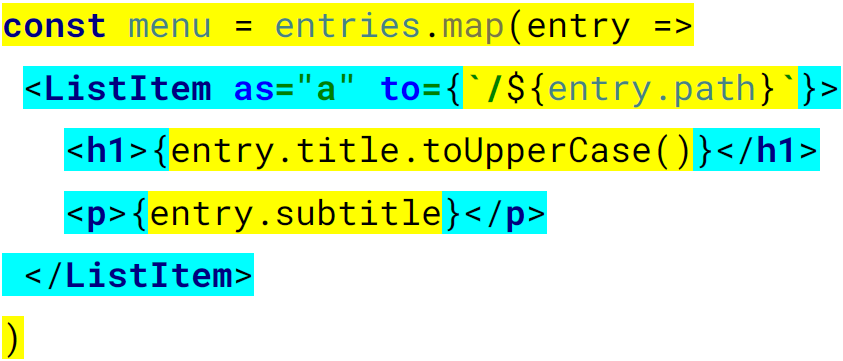
\includegraphics[width=0.6\linewidth]{img/react_jsx.png}\\
\textbf{Styles:} werden nicht als Strings sondern als Object angegeben.

\subsubsection{Conditionals}
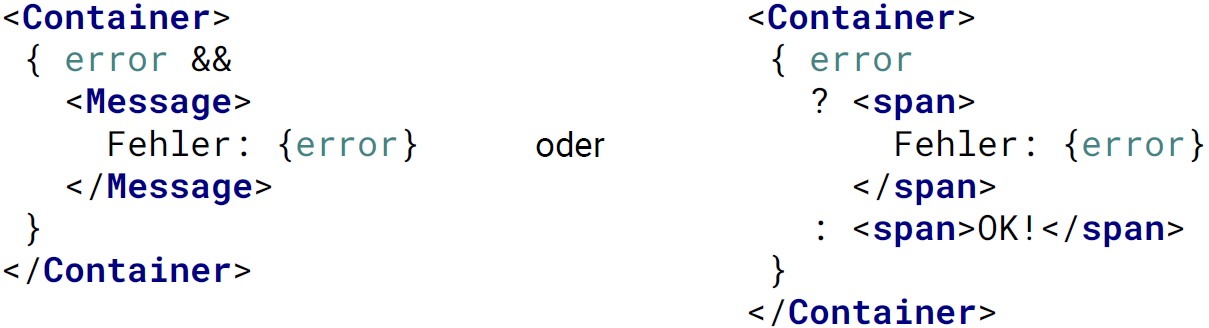
\includegraphics[width=0.7\linewidth]{img/react_jsx_conditionals.png}

\subsubsection{Props}
Komponenten erhalten alle Parameter/Properties als \textbf{props} Objekt.
\begin{itemize}
    \item $this.props$ bei Klassen
    \item Bei Funktionen als Parameter
    \item Immer \textbf{read-only}
\end{itemize}

\subsubsection{Rendering und Mounting}
\textbf{Mounting:} nötig um Komponenten auf Webseite anzuzeigen. \textit{ReactDOM.render}
\begin{lstlisting}
ReactDOM.render(
    <App/>
    document.getElementById('root')
)
\end{lstlisting}

\subsection{React State}
React-Klassenkomponenten können einen veränderbaren Zustand haben.
Der \textbf{state} einer Komponente ist immer privat.
Ändert der State, wird auch die Komponente aktualisiert.
\begin{lstlisting}
class Counter extends React.Component {
    state = { counter: 0 }
    // ...
}
\end{lstlisting}

\subsubsection{Event Handler}
\begin{lstlisting}
const increment = () => {
    this.setState({counter: this.state.counter + 1})
} // ...
<button onClick={this.increment}>
\end{lstlisting}

\subsection{Reconciliation}
\begin{enumerate}
    \item React Komponenten werden als virtueller DOM gerendert
    \item Wird der \textbf{state} geändert, erstellt React einen virtuellen DOM
    \item Alter und neuer DOM werden verglichen
    \item Erst dann werden geänderte DOM-Knoten im Browser erstellt
\end{enumerate}